\title{Singularity Software}
\date{\today}

\documentclass[12pt]{article}
\usepackage[a4paper]{geometry}
\usepackage{lscape}
\usepackage{amsmath}
\usepackage{graphicx}
\usepackage[final]{pdfpages}
\usepackage{grffile}

\geometry{top=1.0in, bottom=1.0in, left=1.0in, right=1.0in} % Sets the margins

\setlength{\parindent}{0pt} % Fixes the paragraph spacing problem

\renewcommand*\arraystretch{1.5}

\begin{document}
\vspace*{\fill}
        \begin{center}
                \LARGE{Siftables Emulator} \\
                \LARGE{\textit{Singularity Software}} \\
                Milestone 5 \\
                \vspace{.15in}
                \large{\today} \\
                \vspace{4in}
                        Alex Mullans \\
                        Ethan Veatch \\
                        Eric Vernon \\
                        Kurtis Zimmerman
        \end{center}
\vspace*{\fill}
\thispagestyle{empty}

\clearpage

\tableofcontents

\clearpage

\section{Project Background}
The Siftables Emulator is being developed by Singularity Software as part of the Junior Project sequence of classes at Rose-Hulman Institute of Technology. When projects were solicited for the sequence, clients Tim Ekl and Eric Stokes (both Rose-Hulman alumni) submitted a request for an emulator for Sifteo Cubes, a new platform intended for ``intelligent play." After Singularity was chosen for the project, we met with Mr. Ekl to determine the three primary features of the Emulator: a Workspace where 1-6 Cubes could mimic the manipulations possible with physical Cubes, an to program those virtual Cubes, and a set of example games designed to show off the first two features. Singularity's Emulator  is intended to build on the foundation of Sifteo, Inc.'s existing emulator by creating a more fluid and natural user interface.
 \\\\
The clients' only implementation-specific specification was the ability to run the finished emulator on a Mac.

\clearpage

\section{Analysis Models}

\subsection{System Sequence Diagram}
The initial RunProgram system sequence diagram had a duplicate step which was annihilated by replacing the \textit{FileOpened} result with the \textit{RunningWorkspace} result because the two were essentially duplicates.

\begin{center}
        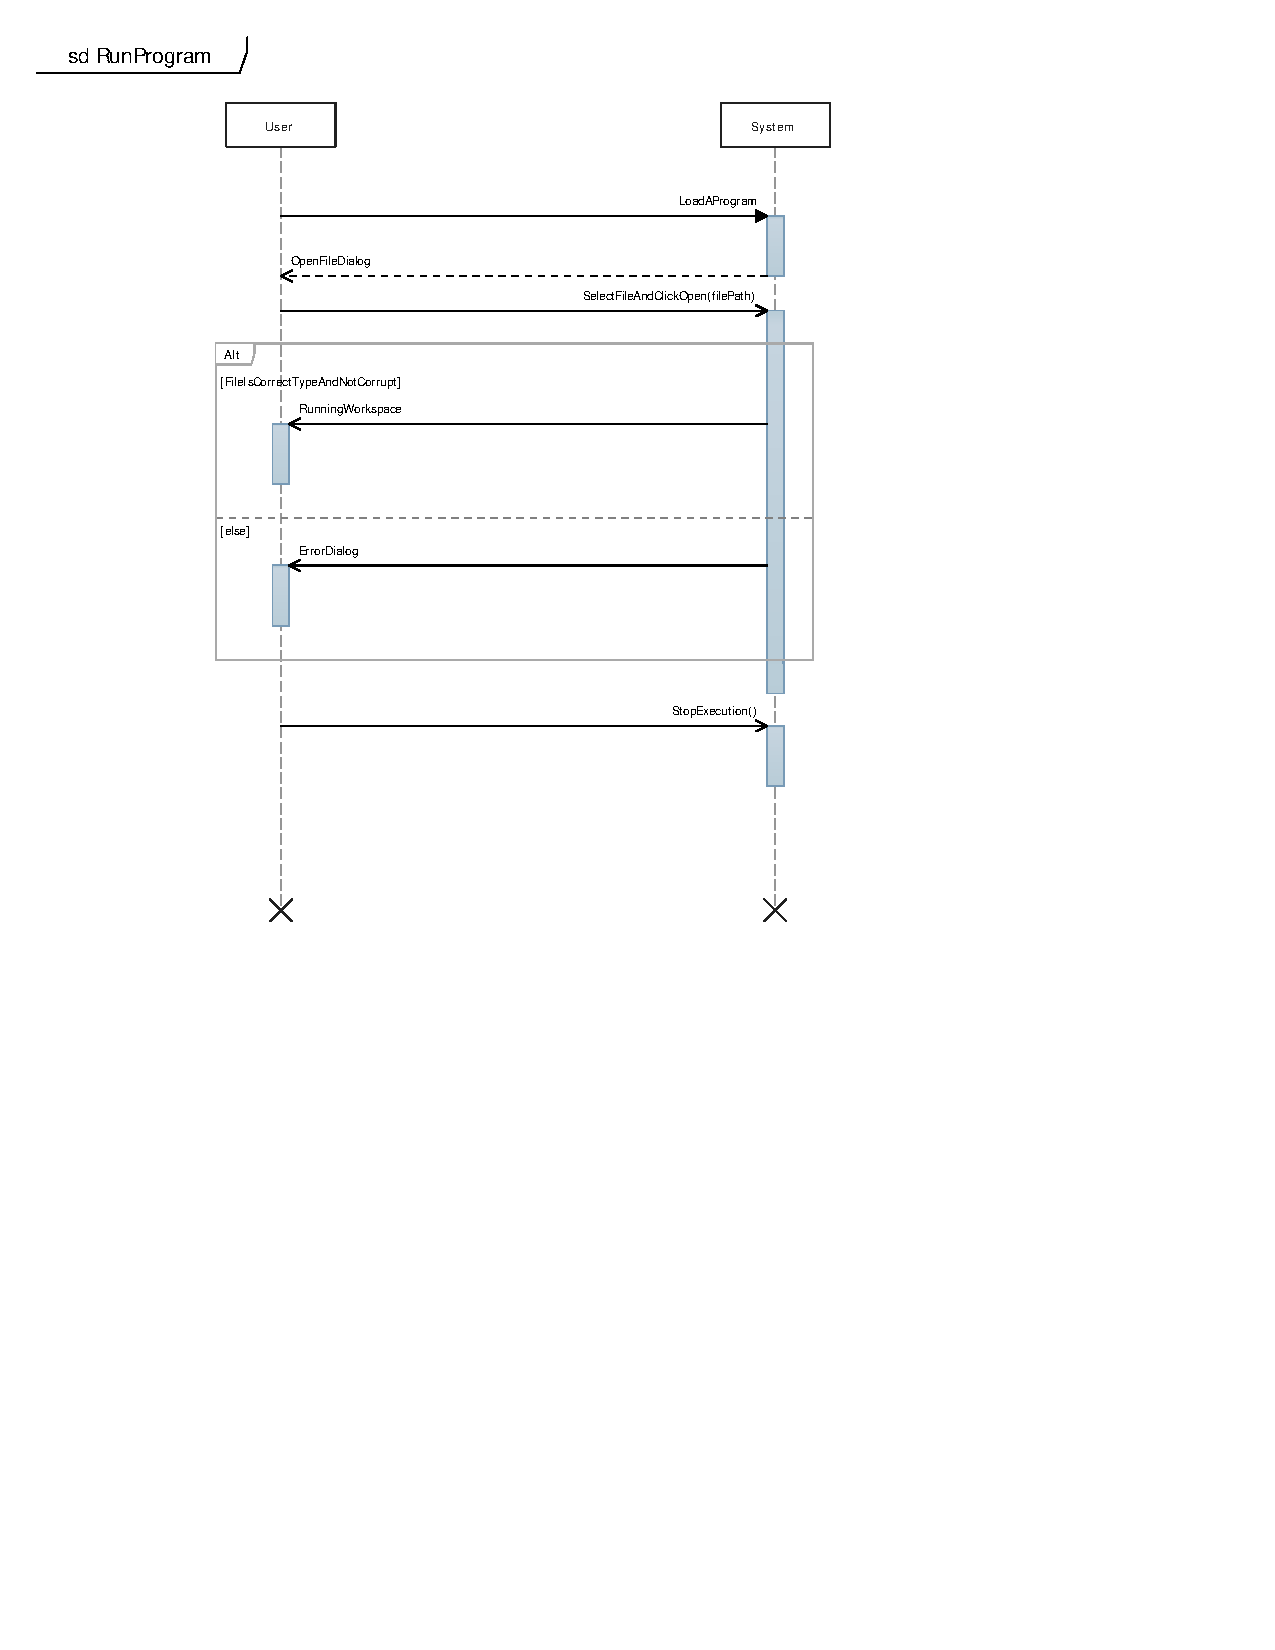
\includegraphics[scale=1]{./pdfs/MS4Models/LoadProgram.pdf}
\end{center}

\subsection{Sequence Diagrams}

\begin{center}
        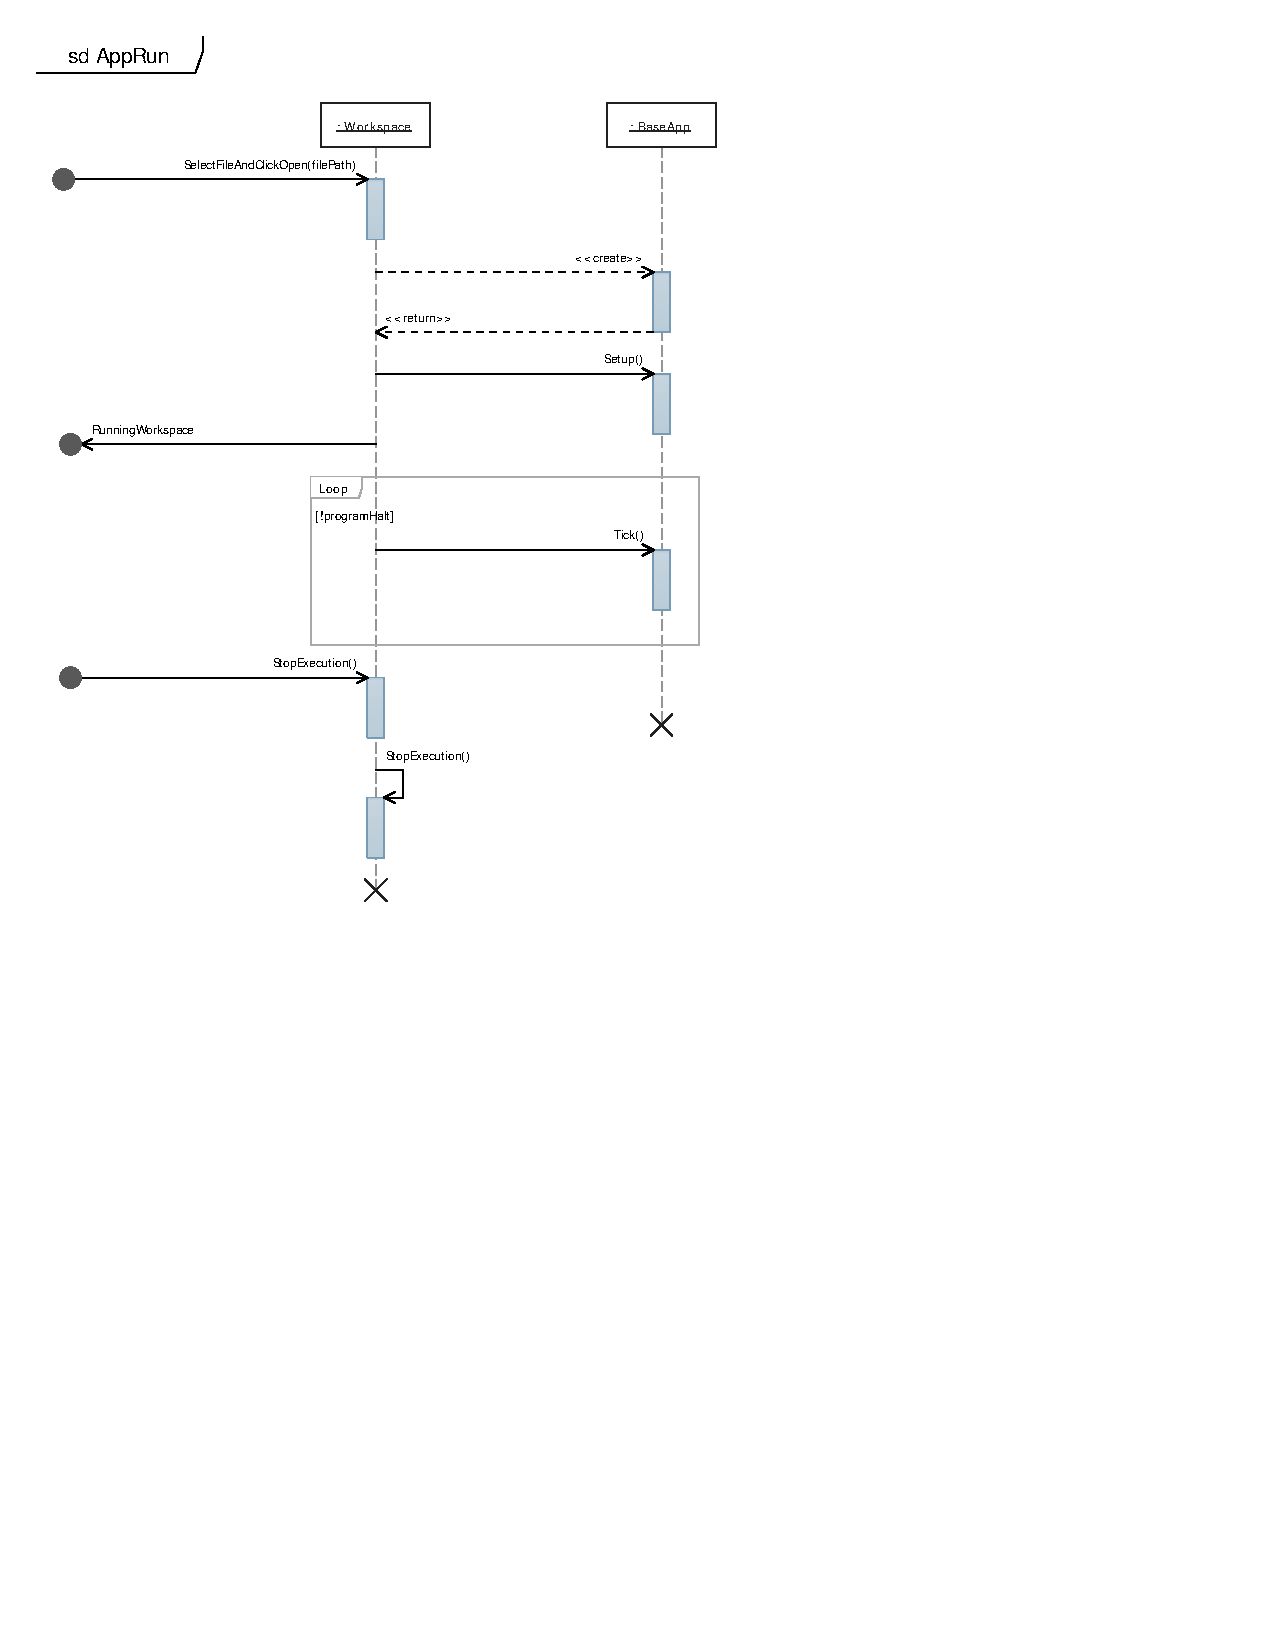
\includegraphics[scale=1]{./pdfs/MS4Models/ReflexGame.pdf}
\end{center}
The \textit{Setup()} operation is necessary in addition to a constructor because this is the way in which initialization of an application is handled per Sifteo's API. No changes were made to this sequence diagram because it is consistent with the way in which the system behaves during this operation.

\begin{center}
        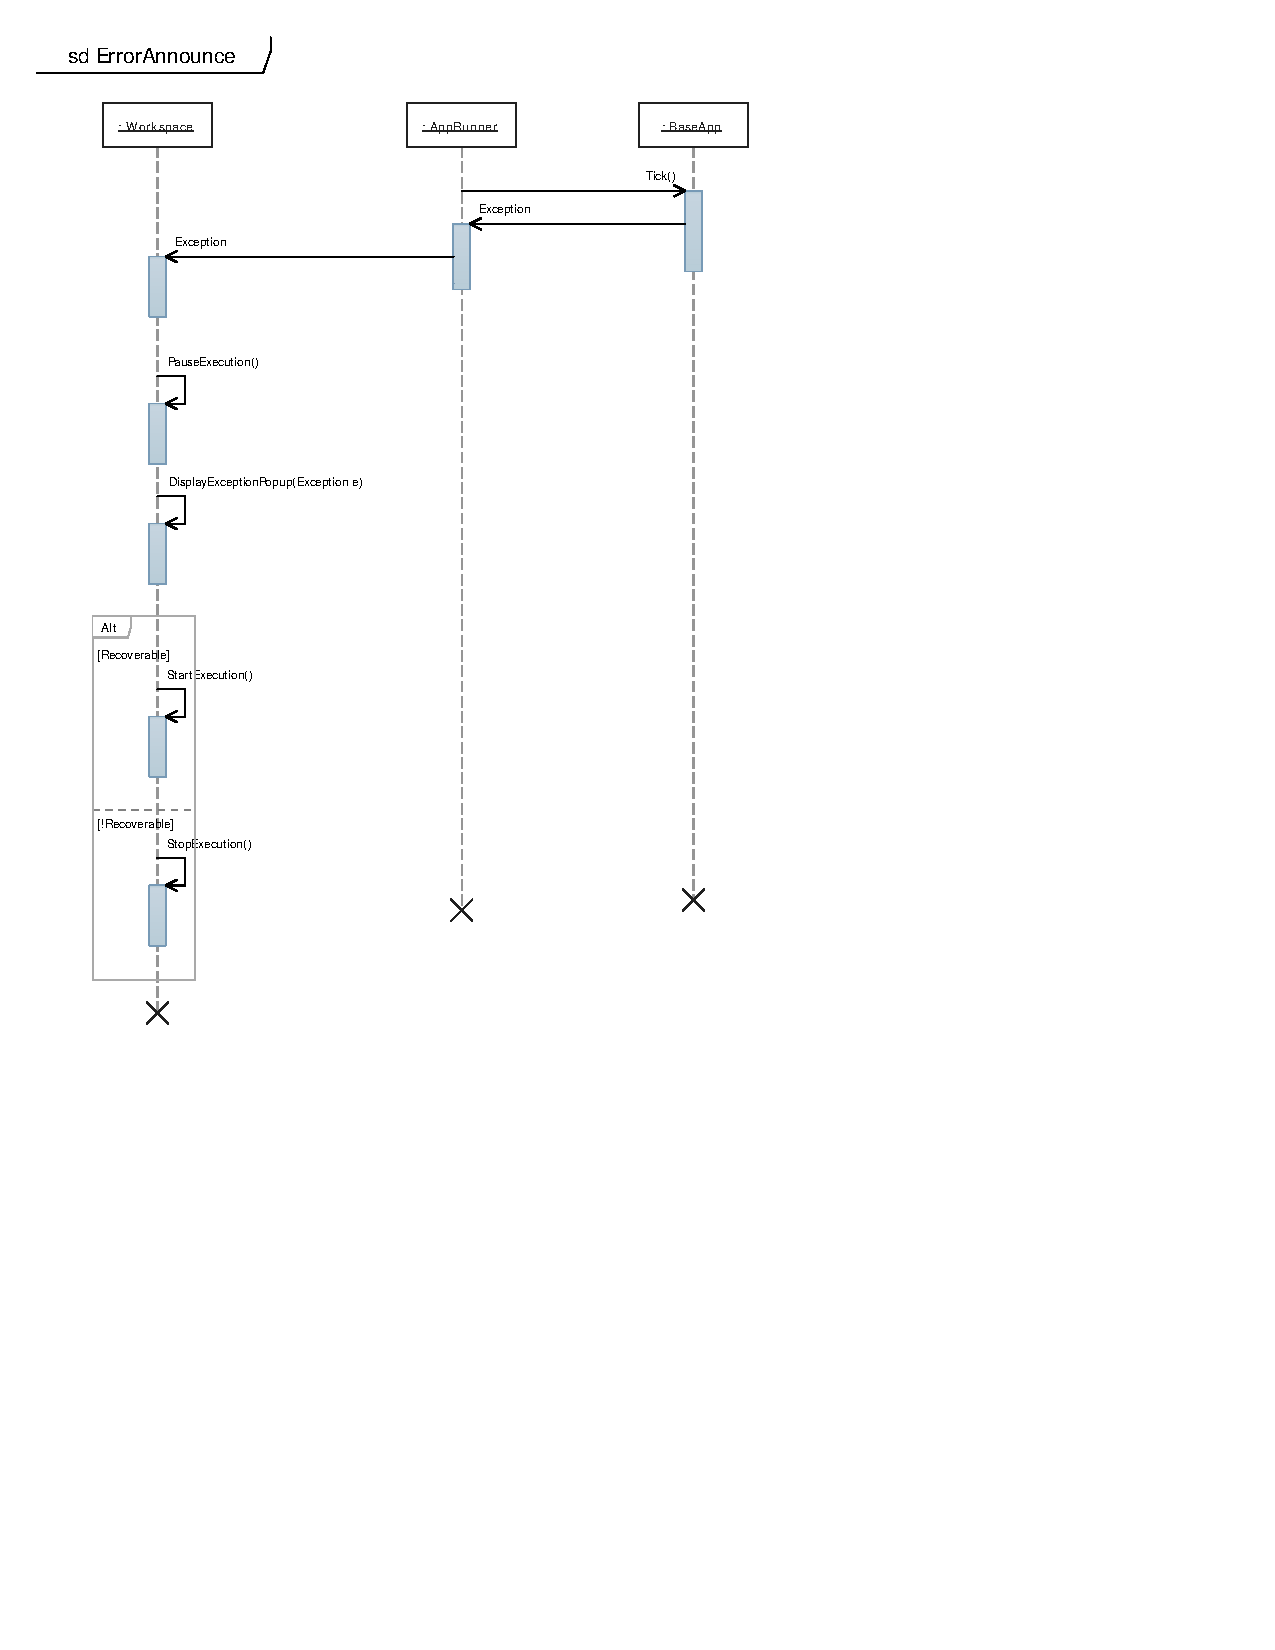
\includegraphics[scale=1]{./pdfs/MS5Models/ErrorAnnounce.pdf}
\end{center}
The \textit{Tick()} operation was unintentionally omitted from the original diagram, and it has been added for clarity to indicate that the action is taking place during an actively running application.

\clearpage

\subsection{Activity Diagram}
The following activity diagram details the process beginning with the user loading a program to the point at which the user closes the program.

\begin{center}
        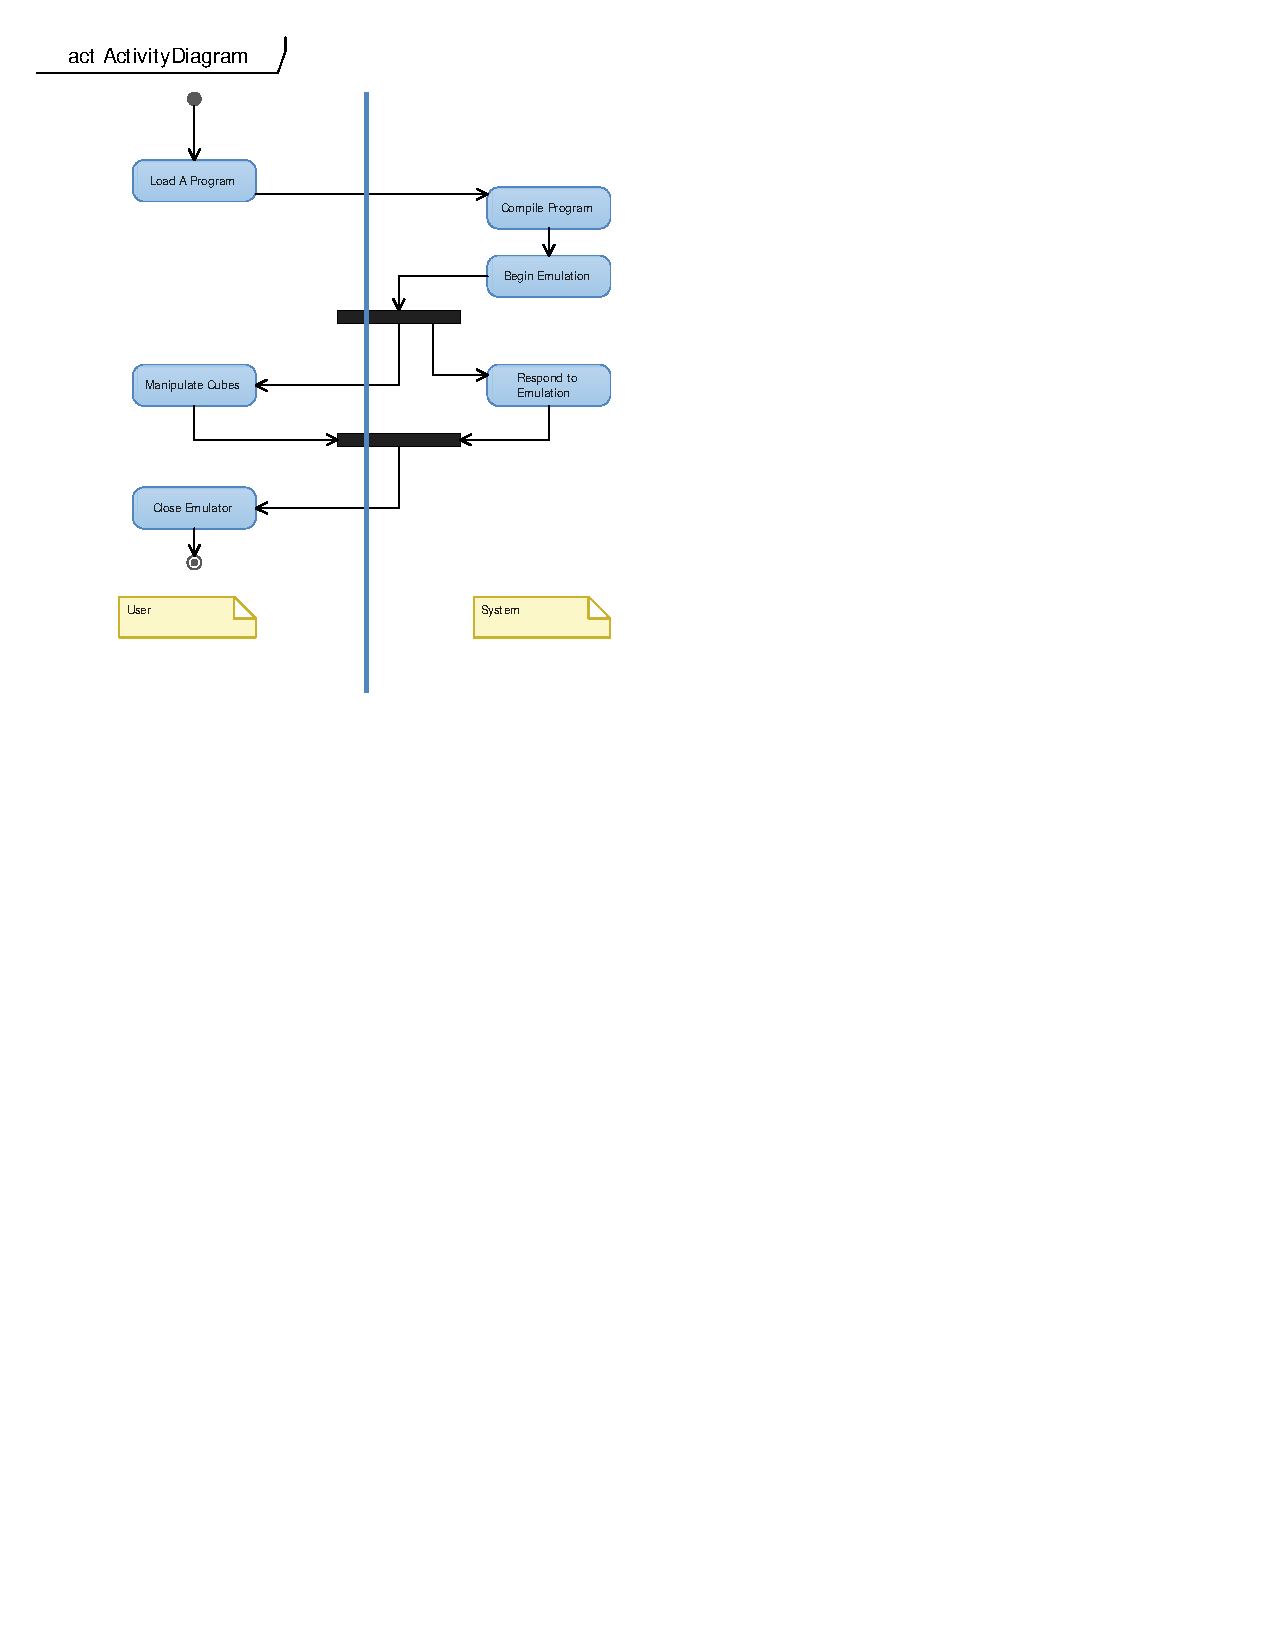
\includegraphics[scale=1]{./pdfs/MS5Models/ActivityDiagram.pdf}
\end{center}

\subsection{Design Class Diagram}
Any external relationships our shown beneath the class name to emphasize interaction with classes we did not create. For instance, each \textit{Cube} is implemented as a \textit{UserControl} object.
\\\\
Additionally, every entity in our diagram is being implemented in our own original code, though many classes are inspired by the Sifteo API which we have to mirror. Those entities which do mirror the objects in the Sifteo domain will be separated into a distinct package to clarify the divide between those objects which carry out the emulation and those which the user primarily manipulates in their original applications.

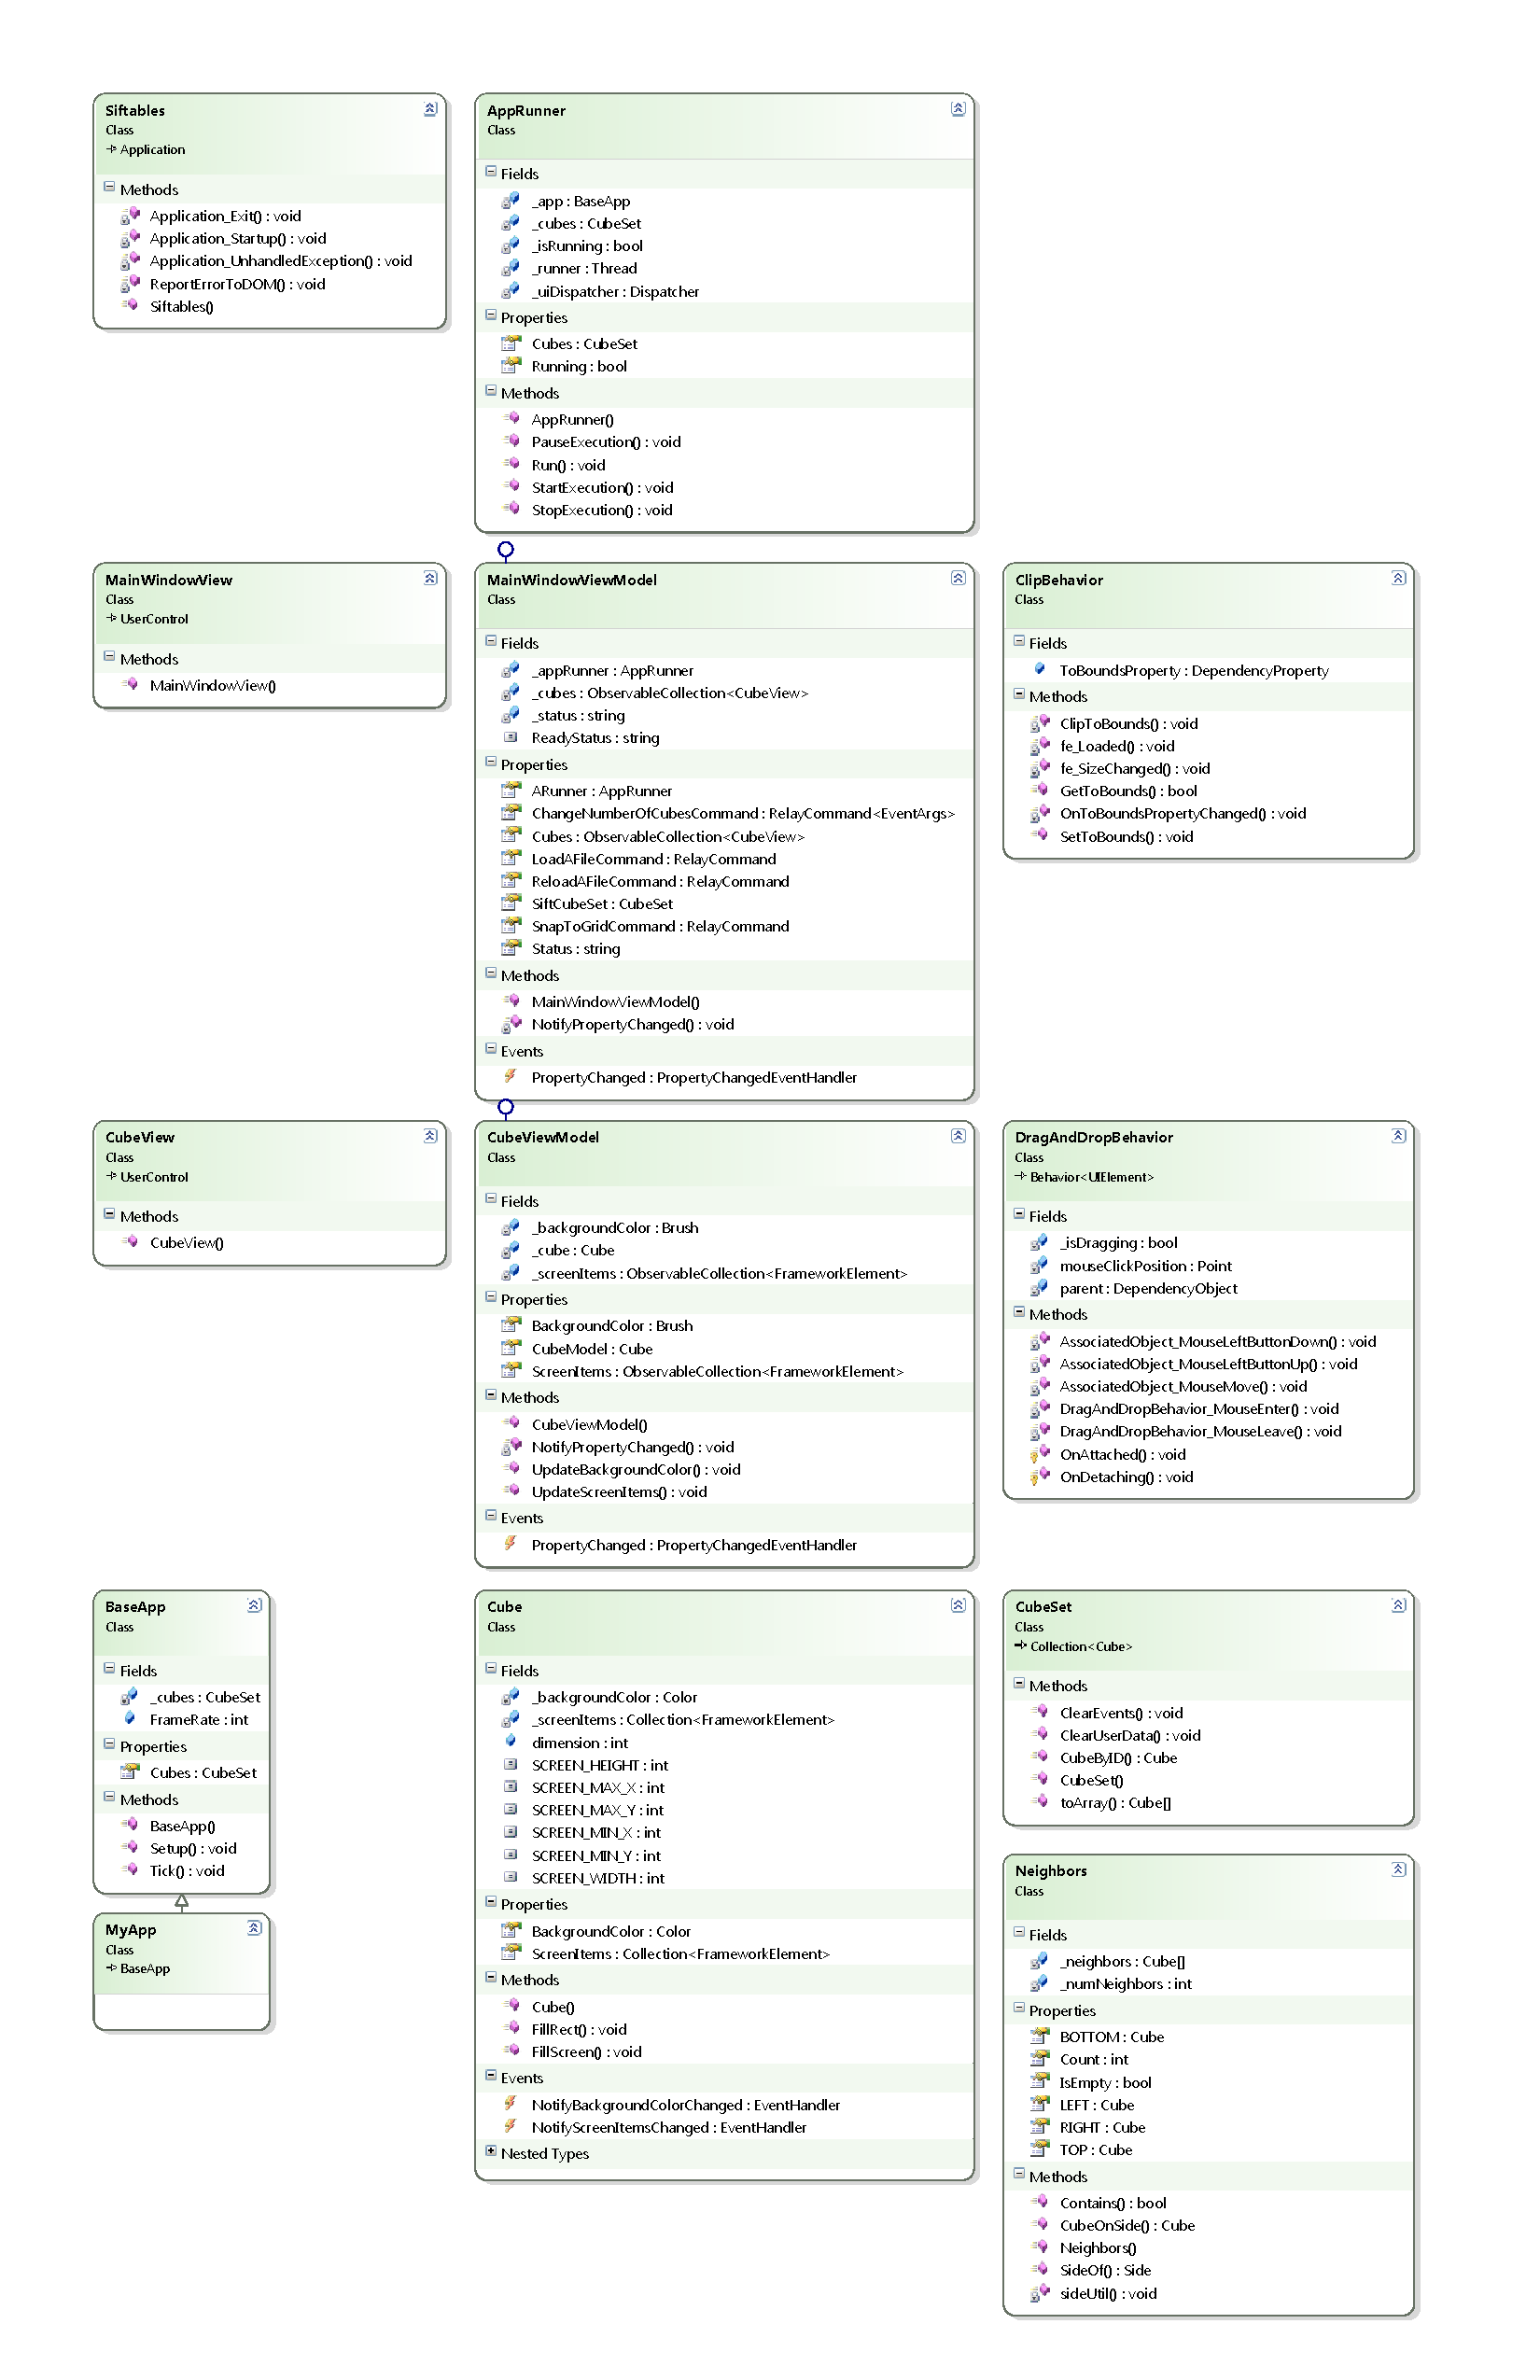
\includepdf{./pdfs/MS5Models/ClassDiagram.pdf}

\textbf{Note}: Because the class diagram was generated by Visual Studio, no associations were created (for instance, between the entity \textit{Cube} which is associated with a unique \textit{Neighbors} entity). We feel no clarity was lost by ommitting these associations.

\section{Applications of the GoF Principles}

\subsection{Facade}
The emulator system is designed in such a way that application developers have just one point of entry: the Sifteo API. The developer can only interact via objects like Cubes, CubeSets, etc. as defined in the Sifteo package, and need not (and do not) have any notion of the specific implementation of the interactions between system-level components and the domain objects exposed by the Sifteo API.

\subsection{Observer}
The MVVM framework makes use of the interface INotifyPropertyChanged. The ViewModels have properties, and the changing of those properties is observed by the view, which responds as defined in the user interface. The use of bindings and ItemsControl objects allows the views to "observe" the ViewModels and their properties or observable collections. This supports loose coupling by abstracting the ViewModel away from the view so the view logic can be implemented independent of the final view.

\subsection{Singleton}
One instance of an AppRunner will be created, and when an application is loaded by the user it is associated with the AppRunner, along with the current CubeSet in the environment. If there were more than one AppRunner in the emulator workspace, then multiple applications could end up running and causing inconsistencies in the expected execution and the visual output in the workspace. Having AppRunner as a Singleton removes this potential inconsistency.

\clearpage

\section{Acceptance Test Plan}
The test cases included in this section are integration tests that simultaneously serve as acceptance tests for the user interface. Because the user interface is the focal point of the project, a functional user interface reasonably exemplifies a functional project. In the future, it may become necessary to test our implementations of the Sifteo package by adding further acceptance tests.

\subsection{Load program}

\begin{table}[h!]
  \begin{tabular}{l | l | l | l}
    \textbf{Scenario \#} &
    \textbf{Originating Flow} &
    \textbf{Alternate Flow} &
    \textbf{Next Alternate} \\ \hline

    1 &
    Basic flow &
    &
    \\ \hline

    2 &
    Basic flow &
    Alternate flow 1 &
    \\ \hline

    3 &
    Basic flow &
    Alternate flow 2 &
    \\ \hline

    4 &
    Basic flow &
    Alternate flow 3 &
    \\ \hline

    5 &
    Basic flow &
    Alternate flow 4 &
    \\ \hline

    6 &
    Basic flow &
    Alternate flow 4 &
    Basic flow \\ \hline

  \end{tabular}
\end{table}

\begin{table}[h!]
  \begin{tabular}{p{.5in} | p{.75in} | p{2.15in} | p{2.15in}}
    \textbf{Test Case ID} &
    \textbf{Scenario} &
    \textbf{Description} &
    \textbf{Expected Result} \\ \hline

    1 &
    1 &
    A program is successfully loaded in the emulator. &
    The Cubes run the selected program in the Workspace. \\ \hline

    2 &
    2 &
    User selects incompatible file type. &
    ``The selected file is not a proper Siftables application and cannot be loaded.'' error is displayed. \\ \hline

    3 &
    3 &
    User selects corrupt or unloadable file. &
    ``The selected file is corrupt and cannot be loaded.'' error is displayed. \\ \hline

    4 &
    4 &
    User cancels loading program. &
    The emulator returns to its state before the basic flow was entered. \\ \hline

    5 &
    5 &
    User loads a program when a program is already running and chooses ``Cancel'' on the warning prompt. &
    Emulator returns to its state before the basic flow was entered after ``Cancel'' is chosen. \\ \hline

    6 &
    6 &
    User loads a program when a program is already running and chooses ``Continue" on the warning prompt. &
    Cubes run the selected program in the Workspace after ``Continue'' is chosen. \\ \hline
  \end{tabular}
\end{table}
\clearpage

\subsection{Reload program}

\begin{table}[h!]
  \begin{tabular}{l | l | l}
    \textbf{Scenario \#} &
    \textbf{Originating Flow} &
    \textbf{Alternate Flow} \\ \hline

    1 &
    Basic flow &
    \\ \hline

    2 &
    Basic flow &
    Alternate flow 1 \\ \hline

  \end{tabular}
\end{table}

\begin{table}[h!]
  \begin{tabular}{p{.5in} | p{.75in} | p{2.15in} | p{2.15in}}
    \textbf{Test Case ID} &
    \textbf{Scenario} &
    \textbf{Description} &
    \textbf{Expected Result} \\ \hline

    1 &
    1 &
    The program is successfully reloaded in the emulator. &
    The Cubes run the selected program in the Workspace after the user presses ``Continue'' on the warning message. \\ \hline

    2 &
    2 &
    The user selects ``Cancel'' on the warning dialog (which specifies that the emulator will be reset). &
    The Cubes run the program as originally specified; no change should be made to emulator's state. \\ \hline

  \end{tabular}
\end{table}

\subsection{Zoom screen}

\begin{table}[h!]
  \begin{tabular}{l | l}
    \textbf{Scenario \#} &
    \textbf{Originating Flow} \\ \hline

    1 &
    Basic flow \\ \hline

  \end{tabular}
\end{table}

\begin{table}[h!]
  \begin{tabular}{p{.5in} | p{.75in} | p{2.15in} | p{2.15in}}
    \textbf{Test Case ID} &
    \textbf{Scenario} &
    \textbf{Description} &
    \textbf{Expected Result} \\ \hline

    1 &
    1 &
    User zooms in fully. &
    The Workspace view has been zoomed to twice its original size. \\ \hline

    2 &
    1 &
    User zooms out fully. &
    The entire Workspace is visible. \\ \hline

  \end{tabular}
\end{table}

\clearpage

\subsection{Add/remove Cubes}

\begin{table}[h!]
  \begin{tabular}{l | l | l}
    \textbf{Scenario \#} &
    \textbf{Originating Flow} \\ \hline

    1 &
    Basic flow &
    \\ \hline

  \end{tabular}
\end{table}

\begin{table}[h!]
  \begin{tabular}{p{.5in} | p{.75in} | p{2.15in} | p{2.15in}}
    \textbf{Test Case ID} &
    \textbf{Scenario} &
    \textbf{Description} &
    \textbf{Expected Result} \\ \hline

    1 &
    1 &
    The spinbox is changed to an integer in the range [1, 6]. &
    The specified number of Cubes is shown in the Workspace. \\ \hline

  \end{tabular}
\end{table}

\subsection{Snap Cubes to grid}

\begin{table}[h!]
  \begin{tabular}{l | l}
    \textbf{Scenario \#} &
    \textbf{Originating Flow} \\ \hline

    1 &
    Basic flow \\ \hline

  \end{tabular}
\end{table}

\begin{table}[h!]
  \begin{tabular}{p{.5in} | p{.75in} | p{2.15in} | p{2.15in}}
    \textbf{Test Case ID} &
    \textbf{Scenario} &
    \textbf{Description} &
    \textbf{Expected Result} \\ \hline

    1 &
    1 &
    User presses the ``Snap to Grid'' button. &
    The emulator aligns the Cubes in a grid based on their current positions.  \\ \hline

  \end{tabular}
\end{table}

\clearpage

\subsection{Manipulate Cube}

\begin{table}[h!]
  \begin{tabular}{l | l}
    \textbf{Scenario \#} &
    \textbf{Originating Flow} \\ \hline

    1 &
    Basic flow \\ \hline

    2 &
    Alternate flow 1 \\ \hline

    3 &
    Alternate flow 2 \\ \hline

    4 &
    Alternate flow 3 \\ \hline

  \end{tabular}
\end{table}

\begin{table}[h!]
  \begin{tabular}{p{.5in} | p{.75in} | p{2.15in} | p{2.15in}}
    \textbf{Test Case ID} &
    \textbf{Scenario} &
    \textbf{Description} &
    \textbf{Expected Result} \\ \hline

    1 &
    1 &
    The user double clicks on a Cube. &
    The Cube responds as if a screen click occured. \\ \hline

    2 &
    2 &
    The user clicks on one of the buttons on the Cube. &
    The Cube executes and responds to the associated action (flip, rotate, or tilt). \\ \hline

    3 &
    3 &
    The user drags a Cube next to another Cube. &
    The Cube neighbors with the adjacent Cube, and the two recognize each other as neighbors. \\ \hline

    4 &
    4 &
    The user drags a Cube back and forth in a shaking manner. &
    The Cube responds as if shaken. \\ \hline

  \end{tabular}
\end{table}
        
\end{document}
